\normaltrue \difficilefalse \tdifficilefalse
\correctionfalse

%\UPSTIidClasse{11} % 11 sup, 12 spé
\newcommand{\UPSTIidClasse}{12}

\exer{Pompe à palettes  $\star$ \label{C2:06:10}}
\setcounter{numques}{0}
\UPSTIcompetence{C2-06}
\index{Compétence C2-06}
\index{Pompe à palettes}
\ifcorrection
\else
\textbf{Pas de corrigé pour cet exercice.}
\fi

\ifprof
\else
Soit le mécanisme suivant. On a $\vect{AO}=e\vect{i_0}$ et $\vect{AB}=\lambda(t)\vect{i_1}$. De plus $e=\SI{10}{mm}$ et $R=\SI{20}{mm}$. Le contact entre \textbf{0} et \textbf{2} en $B$ est maintenu en permanence (notamment par effet centrifuge lors de la rotation de la pompe).
\begin{center}
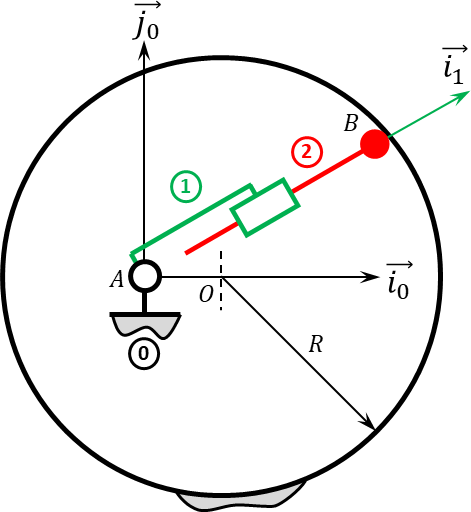
\includegraphics[width=\linewidth]{10_01}
\end{center}
\fi


\question{Tracer le graphe des liaisons.}
\ifprof
\else
\fi

\question{Exprimer $\lambda(t)$ en fonction de $\theta(t)$.}
\ifprof
\else
\fi

\question{Exprimer $\dot{\lambda}(t)$ en fonction de $\dot{\theta}(t)$.}
\ifprof
\else
\fi

\question{Exprimer le débit instantané de la pompe.}
\ifprof
\else
\fi

\question{En utilisant Python, donner le débit instantané de la pompe pour un tour de pompe pour $e=\SI{10}{mm}$ et $e=\SI{15}{mm}$.}
\ifprof
\else
\fi

\question{En utilisant Python, tracer le débit instantané de la pompe pour un tour de pompe pour $e=\SI{10}{mm}$ pour une pompe à 5 pistons (5 branches \textbf{1+2}). On prendra une section de piston \textbf{2} de $\SI{1}{cm^2}$ et une fréquence de rotation de $\dot{\theta}(t)=\SI{100}{rad.s^{-1}}$.}
\ifprof
\else
\fi


\ifprof
\else
\begin{flushright}
\footnotesize{Corrigé  voir \ref{C2:06:10}.}
\end{flushright}%
\fi